%! TEX root = ../thesis.tex
\section{Experiments}%
\label{pdk:sec:experiments}

\begin{table}
	\centering
	\caption{
		Description of datasets used in our experiments.
	}
	\label{pdk:tab:datasets}
	\begin{tabular}{lllrrrr}
		\toprule
		Country     & Type   & Region   & $R$             & $V$            & $K$ & Period     \\
		\midrule

		% Switzerland   & Binary      & Municipality & \numprint{2196} & \numprint{330} & -- & 1981--2020 \\
		% United States & Binary      & State        & \numprint{50}   & \numprint{11}  & -- & 1976--2018 \\
		Switzerland & Binary & Munic.   & \numprint{2196} & \numprint{330} & --  & 1981--2020 \\
		U.S.        & Binary & State    & \numprint{50}   & \numprint{11}  & --  & 1976--2016 \\
		Germany     & Categ. & State    & \numprint{16}   & \numprint{6}   & 5   & 1990--2009 \\
		Germany     & Categ. & District & \numprint{538}  & \numprint{5}   & 5   & 1990--2005 \\

		\bottomrule
	\end{tabular}
\end{table}

We evaluate our algorithm on the four datasets\footnote{The data and the code are available on \href{https://www.github.com/indy-lab/submatrix-factorization}{github.com/indy-lab/submatrix-factorization}.} described in Table~\ref{pdk:tab:datasets}.
The outcomes for the Swiss referenda and for U.S.\ presidential elections are binary.
For Switzerland, this corresponds to the referendum being accepted or rejected.
For the U.S.\, this corresponds to one presidential candidate being elected over the other.
The outcomes for the German legislative elections are one of five categories, corresponding to five political parties.

For the binary datasets, \textit{i.e.}, for Switzerland and for the U.S., we use a GLM~$p$ with univariate Gaussian and Bernoulli likelihoods.
As data about the number of valid votes and about population counts are available for these two datasets, we use a likelihood with weighting, as defined in~\eqref{pdk:eq:weighted}.
For the categorical datasets, \textit{i.e.}, for Germany, we use a GLM with multivariate Gaussian and categorical likelihoods.
As data about population counts were not available in this case, we use a likelihood without weighting, as defined in in~\eqref{pdk:eq:log_likelihood}.

\subsection{Evaluation}

For each dataset, we find the best hyperparameters using the training set only, as explained in details in Appendix~\ref{pdk:app:experimental_setting}.
To evaluate the performance of our algorithm, we compute the mean absolute error (MAE) and the accuracy on the national results.

We first describe the error metrics used for the binary outcome case then extend them for multiple outcomes, \textit{e.g.}, when different parties can be voted.
Let $\vy^* \in \mathbf{R}^R$ be the true regional results and let $\vy \define \vy_{V+1} \in \mathbf{R}^R$ be a prediction.
The true national outcome $y^* \in \mathbf{R}$ is defined as
\begin{equation}
	y^* \define \frac{1}{N} \sum_{r \in [R]} N_r y_r^*,
\end{equation}
where $N = \sum_{r \in [R]} N_r$ is the total number of voters.
The predicted national outcome $y \in \mathbf{R}$ is defined as
\begin{equation}
	y \define \frac{1}{\vert \Ubs \vert} \sum_{r \in \Ubs} N_r y_r + \frac{1}{\vert \Obs \vert} \sum_{r \in \Obs} N_r y_r^*,
\end{equation}
where the prediction $y_r$ in some observed region~$r \in \Obs$ equals the true outcome $y_r^*$.
Then, the MAE and the accuracy of the national prediction are computed as
\begin{align}
	\mae(y, y^*)         & = \vert y - y^* \vert, \label{pdk:eq:mae}                                                                                  \\
	\textrm{Acc}(y, y^*) & = \Indic{y \geq 0.5 \textrm{ and } y^* \geq 0.5} \nonumber + \Indic{ y < 0.5 \textrm{ and } y^* < 0.5}, \label{pdk:eq:acc}
\end{align}
where $\Indic{\cdot}$ is the indicator function.

The MAE enables us to evaluate how far a predictor is from the exact percentage value, whereas the accuracy enables us to evaluate if the outcome is predicted correctly.
For $K$ outcomes, the true and the predicted outcomes are vectors $\vy^* \in [0, 1]^K$ and $\vy \in [0, 1]^K$, respectively, and the MAE in~\eqref{pdk:eq:mae} is simply the $\ell_1$-norm of the difference between the two vectors.
As the accuracy is not defined for multiple outcomes, we compute the average displacement (or Spearman's footrule)~\cite{diaconis1977spearman}.
Let \mbox{$p: [K] \rightarrow [K]$} be a permutation map from a party to its rank for the predicted order, and let \mbox{$p^*: [K] \rightarrow [K]$} be a permutation map for the true order.
The average displacement is then computed as
\begin{equation}
	\label{pdk:eq:displacement}
	D(p, p^*) = \frac{1}{K} \sum_{k=1}^K \vert p(k) - p^*(k) \vert.
\end{equation}
This measures the average position shift between the true rank and the predicted rank of each party.

We train our algorithm on data up to vote $V$ and make predictions on vote $V+1$ to evaluate our algorithm.
To simulate a real setting where results arrive sequentially, we incrementally add regions to the set of observed regions $\Obs$ and average the MAEs on several reveal orders to obtain error bars.
Current political forecasting methods for real-time estimation of the outcomes (\textit{e.g.}, by media outlets) rely mostly on weighted averages of the regional results on the day of the vote.
More sophisticated methods (developed, \textit{e.g.}, by polling agencies) can also be used, but their technical details are not available.
Hence, we compare our algorithm against weighted averaging as a baseline.
For the binary classification task, we also compare against standard matrix factorization (MF) trained with alternating least squares, as proposed by~\citet{etter2016online} and as formulated in Equation~\eqref{pdk:eq:matrix_factorization}.
For the multiple outcome task, we restrict our comparison to weighted averaging.

\subsection{Swiss Referenda}
\label{pdk:sec:swiss_referenda}

We collect a dataset of $V=330$ referenda in $R=2196$ municipalities (the regions are here the municipalities) between 1981 and 2020.
We start with a training set of $V=300$ votes and report the average performance on the next 26 votes with $100$ reveal orders each.
As several votes can occur on the same day, we make sure that only past votes are used in the training set.
In Section~\ref{pdk:sec:depsys}, we analyze in depth the last four votes (two votes on two dates) for which we have real, sequential data.
The ranges of hyperparameters are given in Appendix~\ref{app:ch}, and the best combination for the Bernoulli likelihood is $\lambda = 0.01 $ and $D = 25$.

In Figure~\ref{pdk:fig:ch_results}, we show the MAE and the accuracy of our algorithm to predict national results from partial municipal results.
The two likelihoods used for the GLM provide equal performance, and we report only the performance of the Bernoulli likelihood for clarity.
In terms of MAE (top), MF outperforms the weighted average baseline and our algorithm outperforms MF for every number of observed regions from 1 to 1000.
The difference becomes marginal when more than 1000 results are observed, which suggests that a good approximation of the national result can be obtained by simply averaging the observed results when more than 50\% of the results have arrived.
Nevertheless, in this synthetic setting (the reveal order is randomized) our approach gains only one percentage point at best over the baseline.
In Section~\ref{pdk:sec:depsys}, we will show that the gain becomes substantial with real data, \textit{i.e.}, with the actual reveal order.
In terms of accuracy (bottom), our algorithm predicts the final outcome with 95\% accuracy with 10 observed regions only, outperforming the two baselines by 5 percentage points.
The accuracy of our algorithm reaches 100\% after observing 200 municipal results, \textit{i.e.}, after observing 10\% of all municipalities.

\begin{figure}
	\centering
	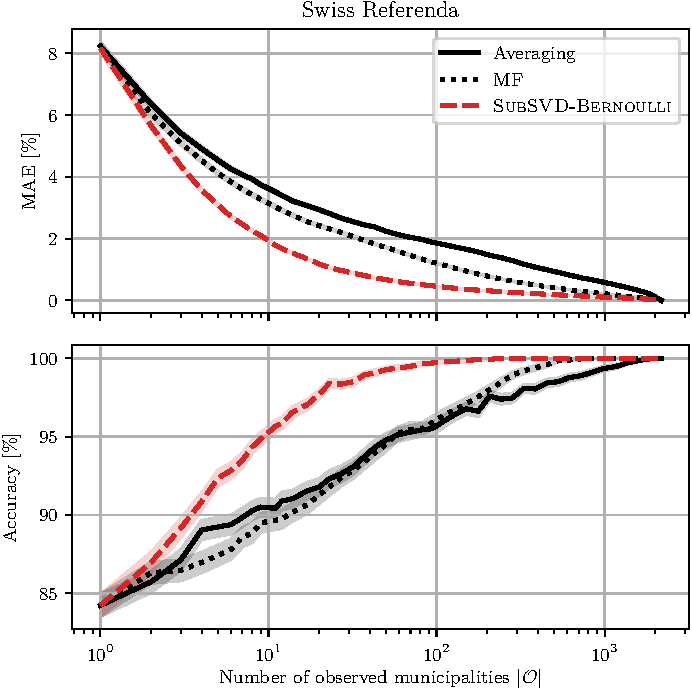
\includegraphics[width=\textwidth*3/4]{pdk-ch-results.pdf}
	\caption{MAE (top) and accuracy (bottom) averaged over 26 Swiss referenda and 100 reveal orders each.}
	\label{pdk:fig:ch_results}
\end{figure}

We explore the patterns in the feature matrix $\vX = \vU \vSigma$ obtained from~\eqref{pdk:eq:projection}.
In Figure~\ref{pdk:fig:ch_svd}, we plot the first two columns of $\vX$, \textit{i.e.}, a projection of the municipalities on the first two singular vectors of the vote representation.
This plot, popularized by~\citet{etter2014mining}, shows two clear clusters of municipalities corresponding to their language.
It also exhibits the infamous \textit{Röstigraben}, a cultural separation between French-speaking municipalities and German-speaking municipalities.
% \footnote{Literally the {\em hash-brown ditch}. It refers to the protective moat set up by the hard-working, frugal, and well-organized Swiss Germans to keep hard-drinking French-speaking leftist rascals at bay.}
In addition, we show in Figure~\ref{pdk:fig:ch_tsne} a projection of the result matrix $\vY$ by using t-SNE~\citep{maaten2008visualizing}.
The language separation is also clearly visible, with French-speaking municipalities on the left of the plot and German-speaking municipalities on the right.
The group of municipalities are further subdivided into smaller clusters corresponding to the canton (states of the Swiss confederation) that they belong to.
Most cantons are uni-lingual in Switzerland, but a few are bilingual.
The most notable among them is Wallis, and interestingly enough, we observe that it is separated into two distinct clusters.
The French-speaking municipalities in Wallis are closer to other French-speaking municipalities, and vice versa for the German-speaking municipalities.
The municipalities of the only Italian-speaking canton, Ticino, form their own cluster.

\begin{figure}
	\centering
	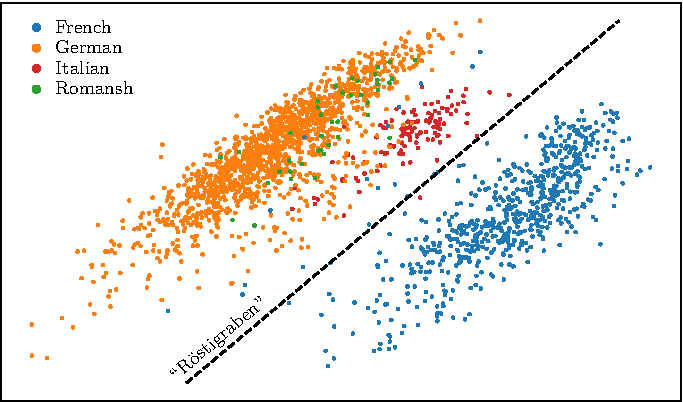
\includegraphics[width=\textwidth*3/4]{pdk-ch-svd.pdf}
	\caption{
		Projection of Swiss municipalities on the first two singular vectors of referendum matrix $\vY$.
		Municipalities are colored according to their language.
	}
	\label{pdk:fig:ch_svd}
\end{figure}

\begin{figure}
	\centering
	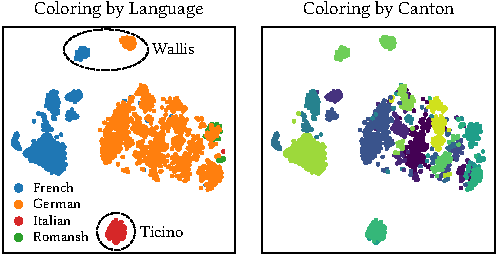
\includegraphics[width=\textwidth*3/4]{pdk-ch-tsne.pdf}
	\caption{
		Projection of Swiss municipalities from referendum matrix $\vY$ with t-SNE.
		(Left) Municipalities are colored according to their language.
		(Right) Municipalities are colored according to their canton (26 cantons).
		The bilingual canton of Wallis is split into two clusters.
		The only Italian-speaking canton of Ticino is isolated from the other clusters.
	}
	\label{pdk:fig:ch_tsne}
\end{figure}

\subsection{U.S.\ Presidential Election}

The U.S.\ presidential election takes place every four years.
We obtain a dataset about the state-level ballots between 1976 and 2016~\citep{mit2017us}.
In the spirit of Nate Silver's \textit{FiveThirtyEight}~\citep{silver2008pollster}, we evaluate the performance of our algorithm at predicting the result of the U.S.\ presidential election in 2016.
The U.S.\ presidential election relies on the electoral-college system, which adds one level of complexity to the prediction because (1) the state-level results are quantized to an integer number of delegates and (2) the candidate who wins the majority of votes in a state wins all the delegates of that state.
This (non-linear) winner-take-all rule requires further modeling assumptions and is out of the scope of this work.
Instead, we focus on predicting the results of the popular vote.

We transform the outcome of the election into a binary outcome of Democratic candidate and Republican candidate.
In all these elections, the results of other parties, \textit{e.g.}, the Green party and independent candidates, are insignificant compared to the two major U.S.\ parties.
This dataset contains the results of $V = 11$ votes in $R = 51$ regions (50 states and the District of Columbia) between 1976 and 2016.
As the number of votes is small, we train our algorithm on all votes up to 2012 ($V = 10$) to set the sub-matrix $\vY_V$, and we predict the state-level results and the national results of the 2016 election.
We report the averaged performance on $10000$ random reveal orders.
The ranges of hyperparameters are given in Appendix~\ref{app:us}, and the best combination for the Bernoulli likelihood is $\lambda = 0.01 $ and $D = 7$.

In Figure~\ref{pdk:fig:us_results}, we show the MAE and the accuracy of our algorithm in predicting this election.
The two likelihoods used for the GLM provide equal performance, and we report only the performance of the Bernoulli likelihood for clarity.
In terms of MAE (top), our algorithm and MF outperform the weighted average baseline after observing the results in two regions.
In terms of accuracy (bottom), our algorithm outperforms both MF and the weighted average for any number of observation.
All models have an accuracy of 41\% after observing the result of one region.
This is because the Democratic candidate won in 21 of 51 regions (41\%) and won the popular vote.

\begin{figure}
	\centering
	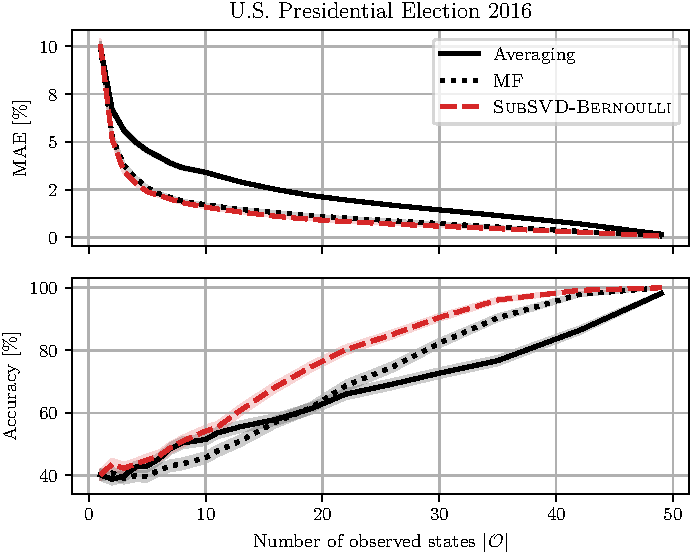
\includegraphics[width=\textwidth*3/4]{pdk-us-results.pdf}
	\caption{MAE (top) and accuracy (bottom) of the popular vote of the U.S.\ presidential election in 2016.}
	\label{pdk:fig:us_results}
\end{figure}

\subsection{German Legislative Election}

German legislative elections take place every four years.
We obtain two datasets~\cite{norsk2020germany} of regional results with $R=16$ states (1990--2009) and $R=538$ districts (1990--2005).
After 2005 (for the districts) and 2009 (for the states), the data are regrettably not publicly available any longer.
We keep $K = 5$ political parties, corresponding to the five major parties in Germany\footnote{CDU/CSU (christian democracy), SPD (social liberalism), FDP (conservative liberalism), the Green party (ecological), and the Left party (radical left).} for which we have data over the whole period.
The datasets cover $V=6$ votes for state-level results and $V=5$ for district-level results.
As there are multiple outcomes, we use a categorical likelihood to predict the results of the five parties.

For the state-level results, we train our algorithm on all votes up to 2005 ($V = 5$) to set the sub-matrix $\vY_V$, and we predict the national results of the 2009 election.
For the district-level results, we train our algorithm on all votes up to 2001 ($V = 4$), and we predict the national results of the 2005 election.
In Figure~\ref{pdk:fig:de_results}, we show the performance of our algorithm in predicting these two elections.
For both datasets, our algorithm outperforms the baseline already after a small number of observations.
The performance for the prediction of the national results when using the fine-grained district-level results is better than when using coarser-grained state-level results.
Remarkably, after observing the results in 10 districts (Figure~\ref{pdk:fig:de_results}, top right), \textit{i.e.}, approximately the average number of districts per state, the MAE reaches 1\%, which is four times better than the MAE obtained after predicting the national outcome from one state (Figure~\ref{pdk:fig:de_results}, top left).
A similar observation can be made for the average displacement.
This suggests that the finer the level of granularity of regions is, the better the predictive performance is, even if the observed results are obtained from the same number of voters.

\begin{figure}
	\centering
	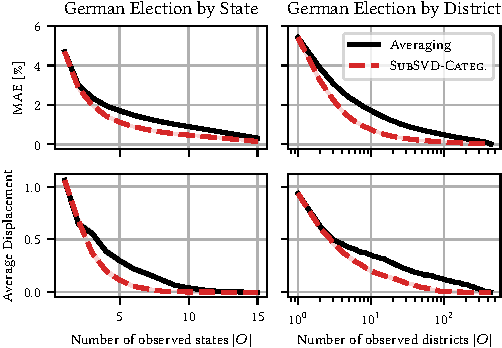
\includegraphics[width=\textwidth*3/4]{pdk-de-results.pdf}
	\caption{MAE (top) and average displacement (bottom) of German legislative elections at state level in 2009 (left) and district level in 2005 (right).}
	\label{pdk:fig:de_results}
\end{figure}

Like with Switzerland in Section~\ref{pdk:sec:swiss_referenda}, we explore the representations of the regions contained in the feature matrix $\vX$ for Germany.
In Figure~\ref{pdk:fig:de_svd}, we plot the first two columns of $\vX$, \textit{i.e.}, a projection of the districts on the first two singular vectors of the vote representations.
We color the points according to the first party elected in the corresponding districts (left).
With no exception, either the CDU/CSU or the SPD is elected.
The two clusters are each separated in half:
The districts on the right side of their cluster vote in majority for the CDU/CSU.
For the lower cluster, those districts also belong to Southern Germany.
The districts on the left side of this cluster (which vote in majority for the SPD) belong to North-Western Germany.

\begin{figure}
	\centering
	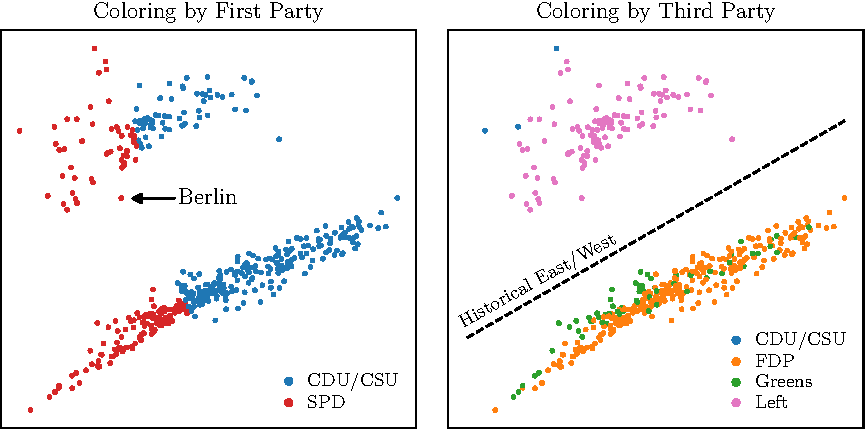
\includegraphics[width=\textwidth*3/4]{pdk-de-svd.pdf}
	\caption{
		Projection of German district on the first two singular vectors of election matrix $\vY$.
		(Left) Districts are colored according to the first party elected in each of them.
		(Right) Districts are colored according to the third party elected.
		This coloring reveals the historical East/West separation.
	}
	\label{pdk:fig:de_svd}
\end{figure}

The CDU/CSU and the SPD have the top two ranks in all districts.
Therefore, it is interesting to color the points according to the party in third place.
This clearly separates the two clusters.
The cluster at the top corresponds to the Left party.\footnote{The three exceptions with CDU/CSU voted the Left party in second place.}
The top cluster contains only districts that belong to historical East Germany (formerly the GDR, before the reunification in 1990), such as Potsdam, Leipzig, and Dresden.
The cluster at the bottom corresponds to the Green party and the FDP and contains only districts that belong to historical West Germany (the former BDR), such as Frankfurt, Munich, and Hamburg.
Interestingly, Berlin lies in the cluster that corresponds to historical East Germany, but seems slightly isolated.
